%!TEX root = ../main.tex

\begin{figure}[ht]
	\centering
	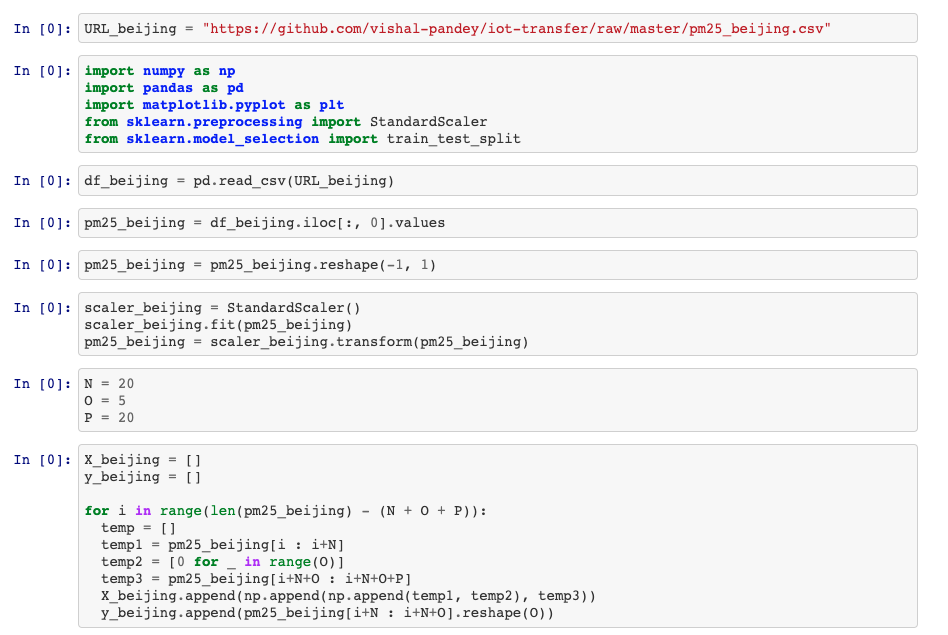
\includegraphics[width=\textwidth]{code/1}
	\caption{Code Screenshot 1}
	\label{fig:code1}
\end{figure}

\begin{figure}[ht]
	\centering
	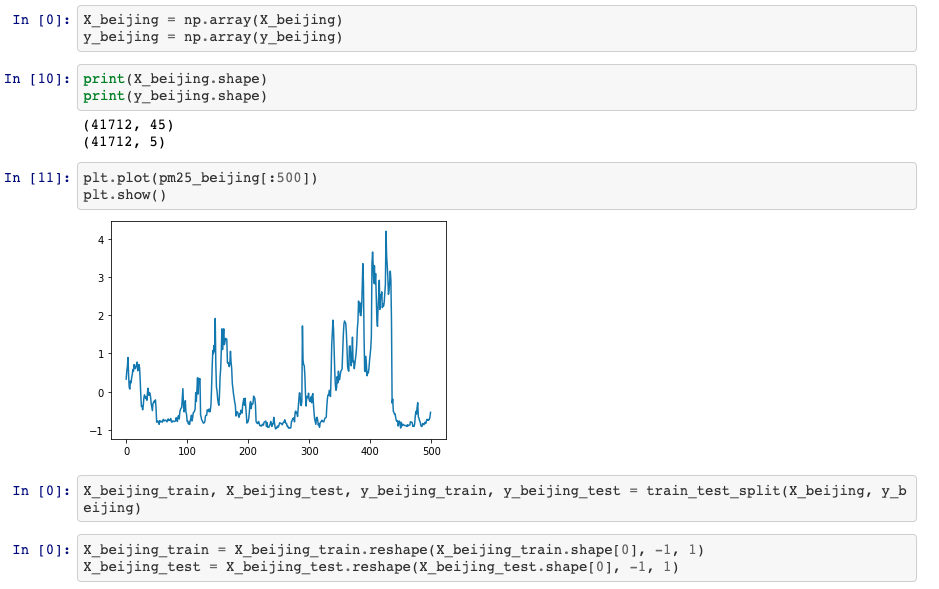
\includegraphics[width=\textwidth]{code/2}
	\caption{Code Screenshot 2}
	\label{fig:code2}
\end{figure}

\begin{figure}[ht]
	\centering
	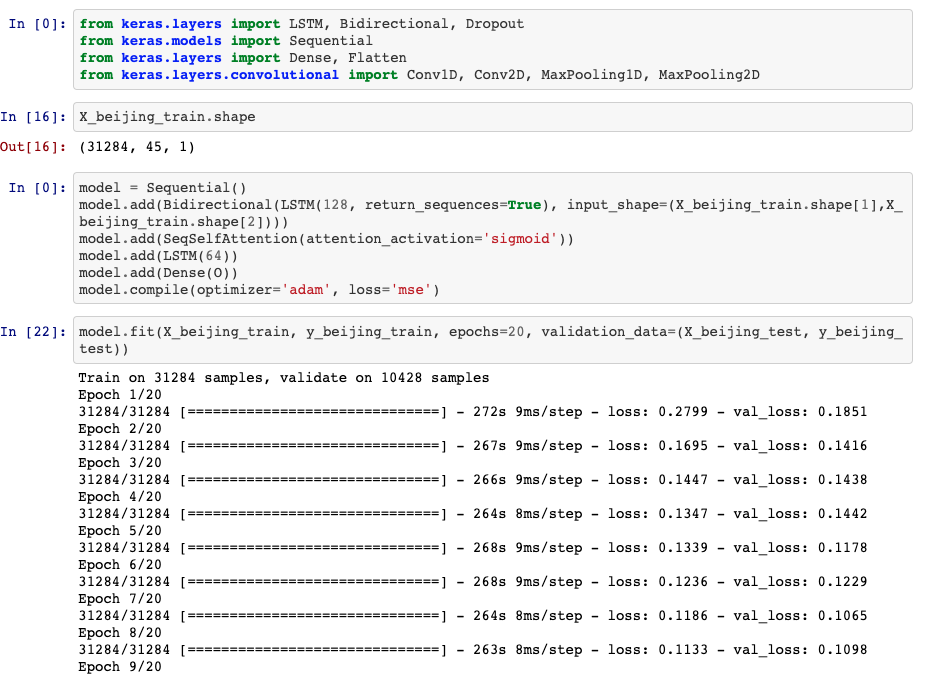
\includegraphics[width=\textwidth]{code/3}
	\caption{Code Screenshot 3}
	\label{fig:code3}
\end{figure}

\begin{figure}[ht]
	\centering
	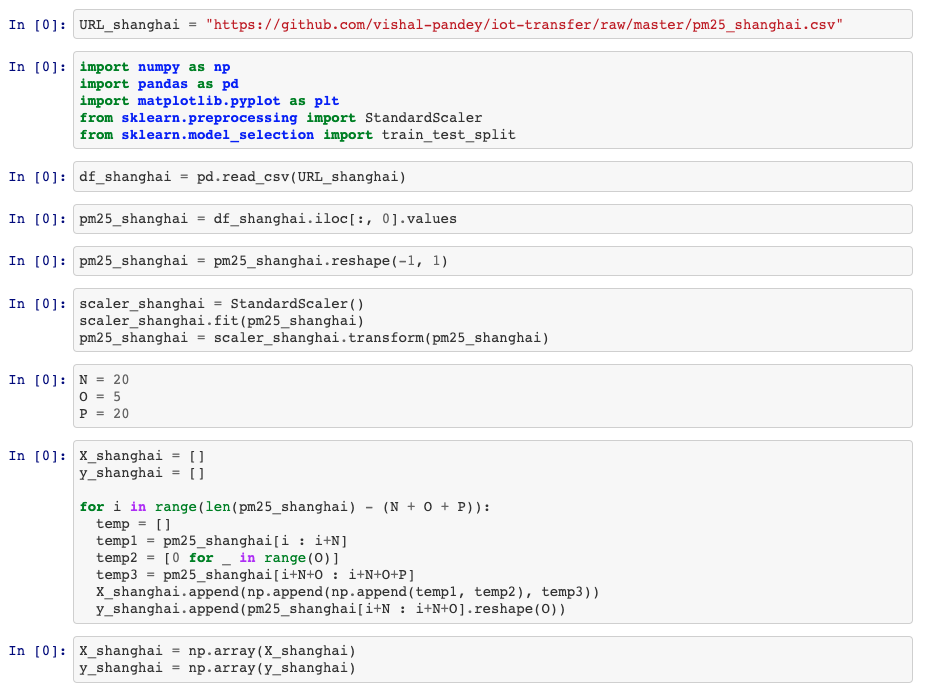
\includegraphics[width=\textwidth]{code/4}
	\caption{Code Screenshot 4}
	\label{fig:code4}
\end{figure}

\begin{figure}[ht]
	\centering
	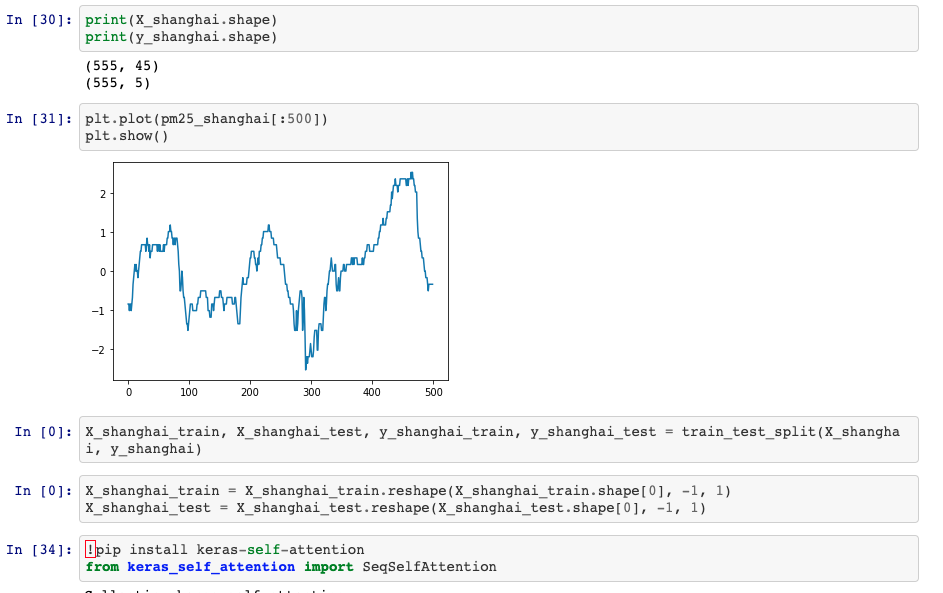
\includegraphics[width=\textwidth]{code/5}
	\caption{Code Screenshot 5}
	\label{fig:code5}
\end{figure}

\begin{figure}[ht]
	\centering
	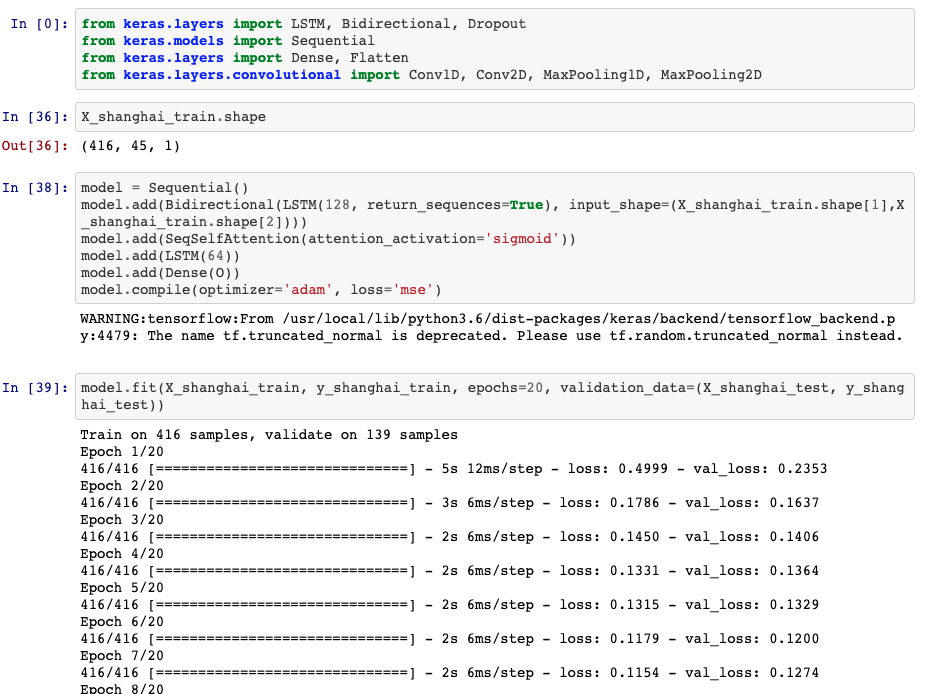
\includegraphics[width=\textwidth]{code/6}
	\caption{Code Screenshot 6}
	\label{fig:code6}
\end{figure}

\begin{figure}[ht]
	\centering
	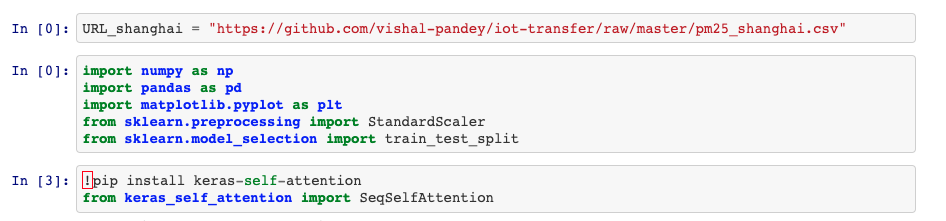
\includegraphics[width=\textwidth]{code/7}
	\caption{Code Screenshot 7}
	\label{fig:code7}
\end{figure}

\begin{figure}[ht]
	\centering
	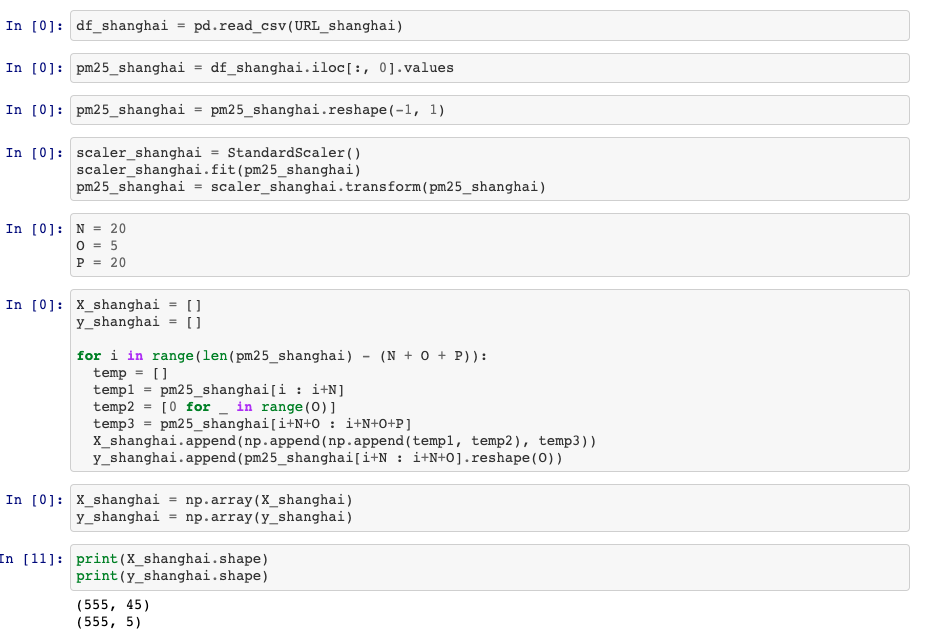
\includegraphics[width=\textwidth]{code/8}
	\caption{Code Screenshot 8}
	\label{fig:code8}
\end{figure}

\begin{figure}[ht]
	\centering
	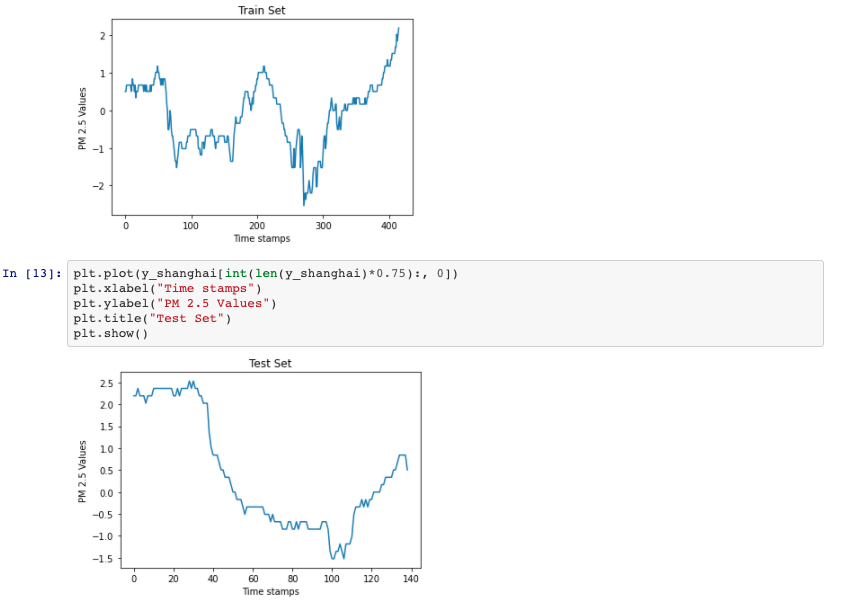
\includegraphics[width=\textwidth]{code/9}
	\caption{Code Screenshot 9}
	\label{fig:code9}
\end{figure}

\begin{figure}[ht]
	\centering
	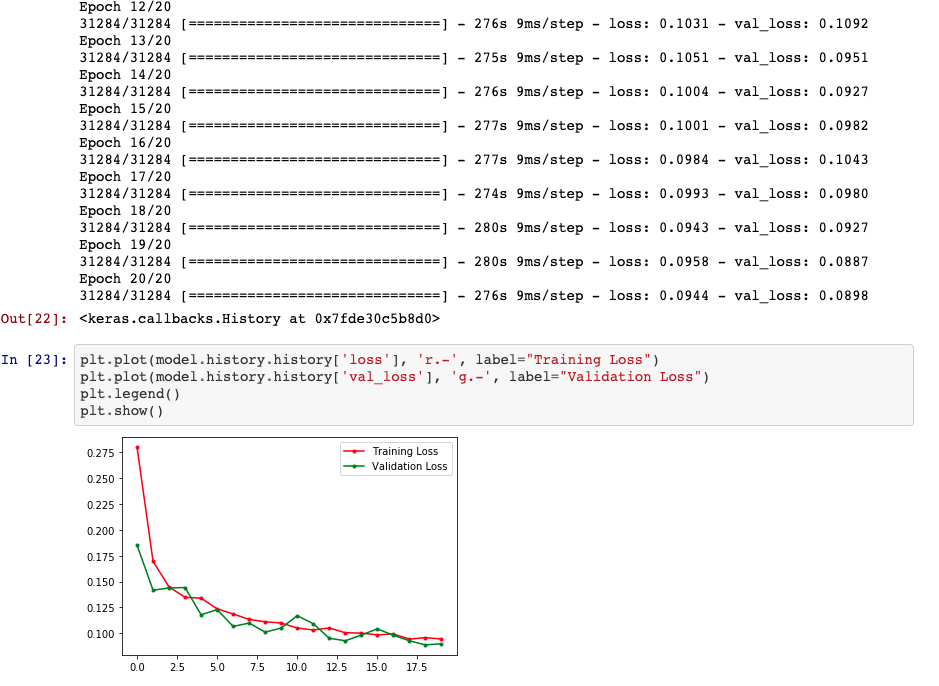
\includegraphics[width=\textwidth]{code/10}
	\caption{Code Screenshot 10}
	\label{fig:code10}
\end{figure}

\begin{figure}[ht]
	\centering
	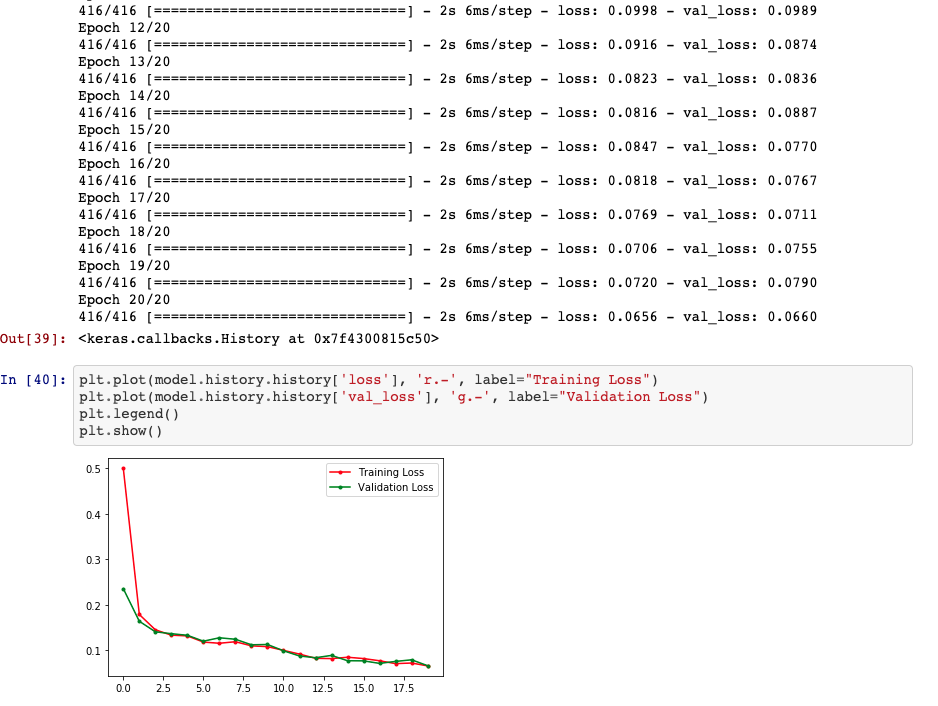
\includegraphics[width=\textwidth]{code/11}
	\caption{Code Screenshot 11}
	\label{fig:code11}
\end{figure}

\begin{figure}[ht]
	\centering
	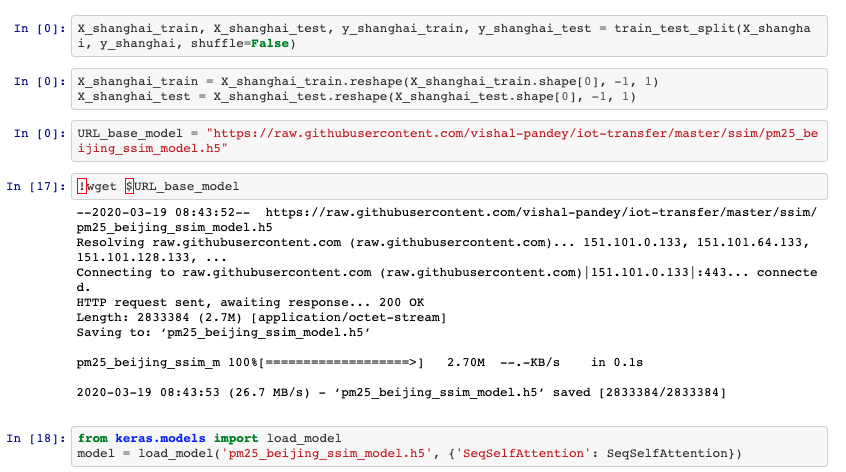
\includegraphics[width=\textwidth]{code/12}
	\caption{Code Screenshot 12}
	\label{fig:code12}
\end{figure}

\begin{figure}[ht]
	\centering
	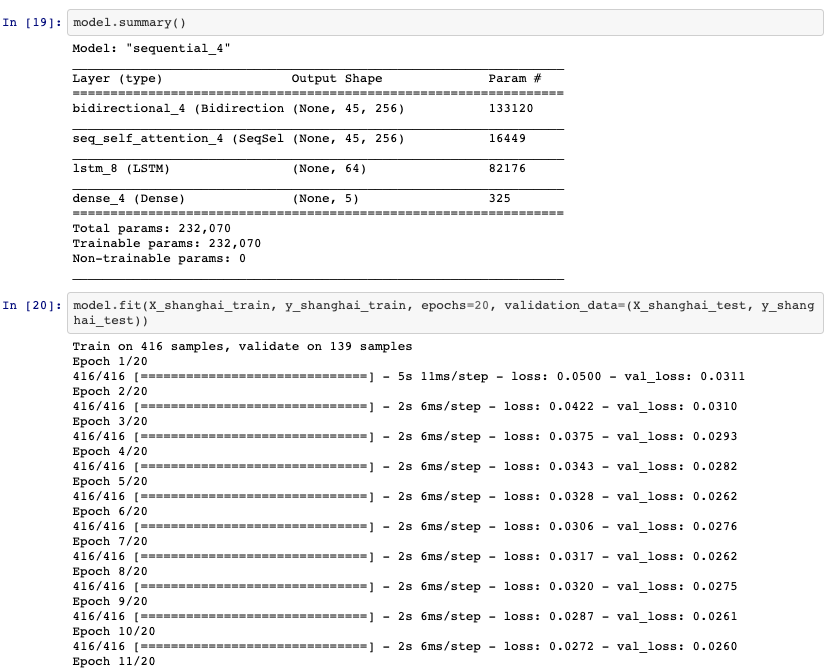
\includegraphics[width=\textwidth]{code/13}
	\caption{Code Screenshot 13}
	\label{fig:code13}
\end{figure}

\begin{figure}[ht]
	\centering
	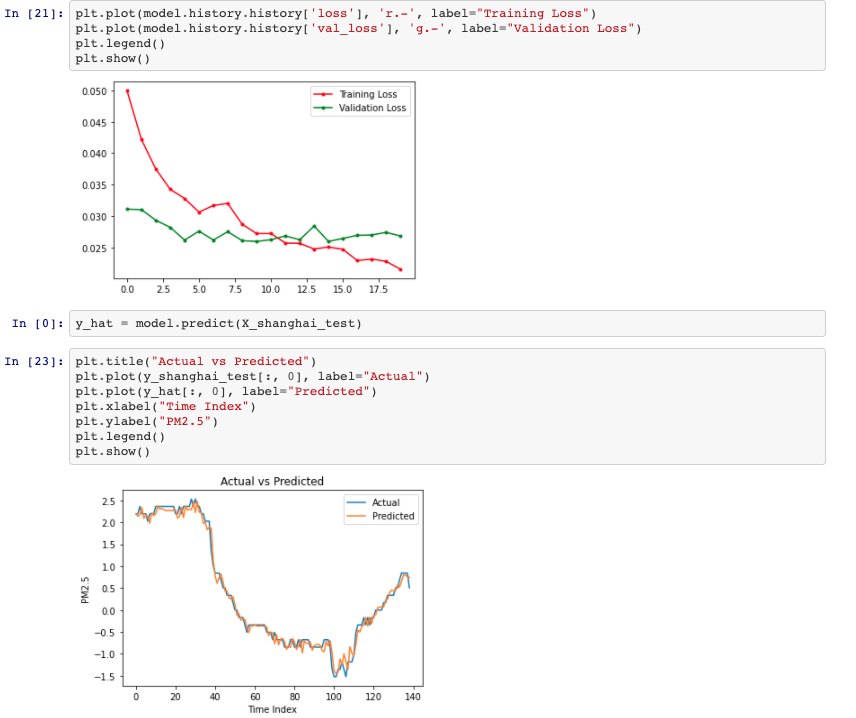
\includegraphics[width=\textwidth]{code/14}
	\caption{Code Screenshot 14}
	\label{fig:code14}
\end{figure}

